% >>>>>>>>>>>>>>>>>>>>>>>>>>>>>>>>>>>>>>>>>>>>>>>>>>>>>>>>>>>
% Dimensions
% <<<<<<<<<<<<<<<<<<<<<<<<<<<<<<<<<<<<<<<<<<<<<<<<<<<<<<<<<<<
\newdimen\topWidth
\newdimen\topHeight
\newdimen\seplineHeight
\topWidth=.31\textwidth
\topHeight=.22\textheight
\seplineHeight=60pt
\setbeamercolor{block body}{bg=sky!10!white,fg=black}
\setbeamercolor{block poster title}{bg=sky!70!white,fg=white}
%
%
%\vfill%
\begin{minipage}[t][\topHeight][t]{\topWidth}%
{\color{BaseDarkColor}\usebeamerfont{block title} Semi-supervised Learning}\\%
Given a finite set of $n$ points $\domain_n\nc\subset\domain\subset\R^d$ with labels $\color{grape}\vec g\nc:\constr_n\nc\subset\domain_n\rightarrow\R$, find a function
\begin{block}{}%
\belowdisplayskip=0pt%
\abovedisplayskip=0pt%
\begin{align*}%
\vec u:\domain_n\nc\to\R,\;\text{ s.t. }\vec u=\color{grape}\vec g \nc\text{ on } \constr_n\nc.
\end{align*}%
\end{block}%
%
\begin{center}%
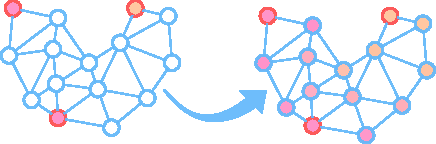
\includegraphics[width=.8\textwidth]{atelier/SSL.pdf}%
\end{center}%
%
{\noindent\color{BaseDarkColor}\usebeamerfont{block title}%
Weighted Graphs}\\%
We model the data as a \alert{weighted graph} $(\domain_n,w_n)$ with edge weights given by
\begin{align*}
w_n(x,y):=
\eta(\abs{x-y}/\scaling_n),\quad x,y\in\domain_n\nc.
\end{align*}
Here $\scaling_n\nc>0$ is a \color{apple}\textbf{scaling parameter}\nc{} and \linebreak $\eta:[0,\infty)\rightarrow[0,\infty)$ is a kernel function.
%
\end{minipage}%
%}%
%
%
\hfill%
%
%
\begin{minipage}[t][\topHeight][t]{0.33\textwidth}%
{\color{BaseDarkColor}\usebeamerfont{block title} Laplacian Learning}\\%
Laplacian learning for $p<\infty$ involves the energy
\begin{align*}
\vec E_p^{w_n}(\vec u) = \sum_{x,y\in\domain_n}w_n(x,y)^p|\vec u(y)-\vec u(x)|^p
\end{align*}
%
and the graph Laplacian
%
{\small%
\begin{align*}
\Delta^{w_n}_p \vec u(x):= \sum_{y\in\domain_n} w_n(x,y)^p \abs{\vec u(y) - \vec u(x)}^{p-2} \left( \vec u(y) - \vec u(x) \right)
\end{align*}
}%
%
%
which yields the equivalent problems:
\vspace{15pt}

%
\begin{minipage}{.45\textwidth}%
\begin{block}{}%
\vbox to 4cm {%
\belowdisplayskip=0pt%
\abovedisplayskip=0pt%
\begin{gather*}
\min_{\vec u} \vec{E}^{w_n}_p (\vec u),\\
\text{ s.t. } \vec u = \color{grape}\vec g\nc \text{ on } \constr_n.
\end{gather*}\vfill}%
\end{block}
\end{minipage}%
\hfill%
$\Leftrightarrow$
\hfill%
\begin{minipage}{.45\textwidth}%
\begin{block}{}
\vbox to 4cm {%
\belowdisplayskip=0pt%
\abovedisplayskip=0pt%
\begin{align*}
\Delta^{w_n}_p\vec u&= 0\text{ in } \domain_n\setminus\constr_n,\\
\vec u &= \color{grape}\vec g\nc \text{ on } \constr_n.
\end{align*}\vfill}%
\end{block}
%
\end{minipage}%
\vspace{.1em}

%
\begin{minipage}{.5\textwidth}%
\centering%
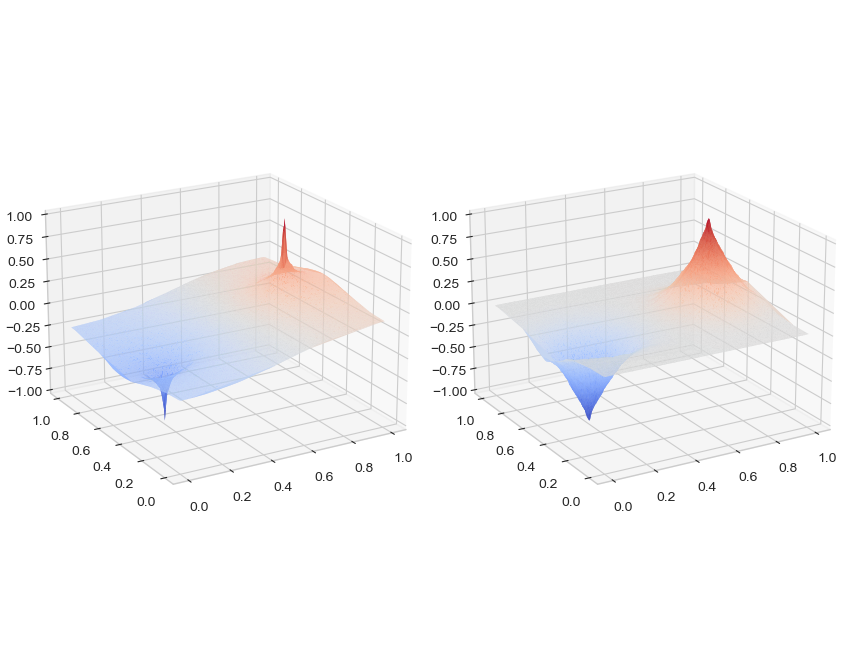
\includegraphics[width=.7\textwidth, trim={0cm 3cm 11cm 4cm}, clip]{atelier/2Dex_50000.png}%
\end{minipage}%
\begin{minipage}{.5\textwidth}%
\alert{Drawback:} In the infinite data limit this problem is only well-posed if $p>d$.
\end{minipage}%
%
%
\vfill%
%
\end{minipage}%
%
%
\hfill%
%
%
\begin{minipage}[t][\topHeight][t]{\topWidth}%
{\color{BaseDarkColor}\usebeamerfont{block title} Lipschitz Learning}\\%
In the limit $p\to\infty$ we obtain the energy
\begin{align*}
\vec E_\infty^{w_n}(\vec u) = \max_{x,y\in\domain_n}w_n(x,y)|\vec u(y)-\vec u(x)|
\end{align*}
%
and the graph infinity Laplacian
%
{\small%
\begin{align*}
\Delta^{w_n}_\infty \vec u(x)
&:= 
\max_{y\in\domain_n} w_n(x,y) \left(\vec u(y) - \vec u(x)\right)
\\
&\qquad
+ 
\min_{y\in\domain_n} w_n(x,y) \left(\vec u(y) - \vec u(x)\right).
\end{align*}}%
%
The associated problems are not equivalent.
%
\begin{minipage}{.45\textwidth}%
\begin{block}{}%
\vbox to 4cm {%
\belowdisplayskip=0pt%
\abovedisplayskip=0pt%
\begin{gather*}
\min_{\vec u} \vec{E}^{w_n}_\infty (\vec u),\\
\text{ s.t. } \vec u = \color{grape}\vec g\nc \text{ on } \constr_n.
\end{gather*}\vfill}%
\end{block}
\end{minipage}%
\hfill%
$\Leftarrow$%
\hfill%
%
\begin{minipage}{.45\textwidth}%
\begin{block}{}
\vbox to 4cm {%
\belowdisplayskip=0pt%
\abovedisplayskip=0pt%
\begin{align*}
\Delta^{w_n}_\infty\vec u&= 0\text{ in } \domain_n\setminus\constr_n,\\
\vec u &= \color{grape}\vec g \nc \text{ on } \constr_n.
\end{align*}\vfill}%
\end{block}
\end{minipage}%
%
\vspace{1em}%

\begin{minipage}{.5\textwidth}%
\centering%
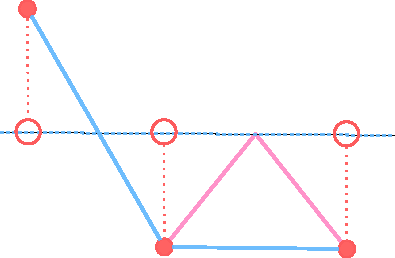
\includegraphics[width=.7\textwidth]{atelier/amle.pdf}%
\end{minipage}%
\begin{minipage}{.5\textwidth}%
Minimizing $\vec E_\infty^{w_n}$ does not admit unique solutions: the blue line shows the~\alert{AMLE}.
\end{minipage}%

\end{minipage}%
\hfill%